\chapter{Our Approach}

Our approach for this project is to use existing frameworks and techniques with proven qualities to analyse the Python source code, most notably the monotone framework. This chapter contains outlines of how these frameworks and techniques are adapted to fit the specific task.

\section{Monotone framework implementation}

To get started an implementation of the monotone framework that is decoupled from the actual analysis was made. This implementation counts commonly used lattice structures, the worklist algorithm, a graph structure and an analysis interface (or trait in scala-lingo).

\subsection{Lattices}
In order to make our lives easier when constructing the actual analysis lattice, we have implemented several common lattice structures as type generic classes. These common lattice structures include, among others, a map and product lattice. In this section we will briefly go over the implementation decisions made for these structures.

Using classic object-oriented programming principles each of these compound structures decide the ordering of their elements by delegating to the underlying lattices in a point wise fashion, e.g. the product lattice has two underlying lattices, one for each element and thus the ordering is decided by comparing the first element in the pair in the context of the first lattice and similarly for the second element.

The map lattice has received a couple of changes from the naive implementation to make it usable in more cases. The first change was to interpret an unbound key value, $k$, to be a mapping from $k$ to the bottom element of the underlying lattice. In some use cases, such as a functional approach to intraprocedural static analysis, the map lattice will have a huge amount of keys. Requiring all of these to be bound to some value in the map is superfluous. This invariant is hidden completely in the lattice class because you can't manipulate the lattice element directly, so when trying to lookup an unbound key, the lattice simply constructs a fresh bottom value.

Since we now have a way to avoid binding every value from the key set, we are also able to change the constructor from the straightforward approach \inlinecode{k: Set[T], v: Lattice[S]} into a more general \inlinecode{k: T, v: Lattice[S]} (where \inlinecode{S} and \inlinecode{T} are type arguments). The straightforward approach has to compute the entire key set before you are able to instantiate the map lattice, but since the key set in itself might be exponentially large that wouldn't be practical. The downside to this change is, that since the map lattice has no way to know the intended key set, there is no way to construct the top element of the lattice.

% The top element of the lattice is useful for when you want to give up in the analysis, so to fix we instrumented the map lattice with a new top element, in a similar fashion to how the sink lattice instruments the underlying lattice with a new bottom element.

\subsection{Constraints}

Being in a functional programming language an easy-to-work-with representation of the constraints is anonymous lambda functions with the type \inlinecode{E $\rightarrow$ E}, where \inlinecode{E} is the type of the elements in the analysis lattice. Each constraint captures the node it was made from in its closure, so it is able to lookup the needed information in the lattice element.

This approach follows the notation very nicely, and as such makes the implementation a simple task when the constraints have been formulated formally.

\subsection{Worklist}
Our worklist implementation hasn't seen any optimizations and is as such just the straightforward implementation. First it generates constraint functions for each of the nodes in the CFG, adding each node to a worklist as it goes along. It then starts recursion (Scala benefits from tail call optimization to prevent the stack from exploding) on the list, popping one node from the list at a time. When a node is popped the corresponding constraint function is applied to the solution. Using Scalas built-in structural equality, the result is compared to the input and if they differ all nodes that depends on the popped node are added to the worklist.

A simple optimization would be to focus on finding a fixed-point for a strongly connected component of the CFG before continuing with the strongly connected components that depend on it, as also explained in section 5.1 from Static Program Analysis \cite{sa}.

\section{The Analysis Lattice}
Inspired by TAJS \cite{tajs} we have constructed a lattice for abstract values, $Value$ (see \autoref{lattice:Value}), from which we build a lattice for abstract objects, $Object$ (see \autoref{lattice:Object}). These two lattices are the main building blocks for the lattice of abstract states, $State$ (see \autoref{lattice:State}). Our analysis lattice is the lattice which for each program point (i.e. for each CFG node) describes the abstract state of that program point. Furthermore the $Analysis$ lattice (see \autoref{lattice:Analysis}) describes the call graph of the CFG.

\subsection{Abstract Values}
The lattice for abstract values follows below:

\begin{figure}[H]
\begin{eqnarray*}
Value = & Undefined \times None \times NotImplemented \times Ellipsis \\
        & \times Boolean \times Integer \times Float \times Long \\
        & \times Complex \times String \times P(ObjectLabel)
\end{eqnarray*}
\vspace{-15pt}
\caption{The $Value$ lattice.}
\label{lattice:Value}
\end{figure}

The $Value$ lattice is used to describe the abstract values of temporary variables, and attributes on objects. The $Undefined$, $NotImplemented$, $Ellipsis$ and $None$\footnote{\inlinecode{NotImplemented}, \inlinecode{Ellipsis} and \inlinecode{None} are examples of built-in constants. See \cite{pyref.constants} for a complete list of built-in constants in Python.} lattices all contain two nodes, top and bottom. $NotImplemented$ is a constant in Python which can be used when a function is not supported. $Ellipsis$ is another constant which represents \inlinecode{\dots} in Python; this constant can be used when indexing using intervals (also known as slicing). When a function does not contain a return statement, the constant \inlinecode{None} is returned by default, e.g.:

\begin{listing}[H]
	\begin{minted}[linenos]{python}
def a(): pass
a() is None # true
	\end{minted}
	\caption{Constant None}\label{code:NoneExample}
\end{listing}

Contrary to JavaScript, Python supports integers, floats, longs and complex numbers, so we have separate lattices for those. As lists in Python can only be indexed using integers our lattices does not have to keep track of whether a particular number is an unsigned integer or not, as the $Num$ lattice for TAJS does (page 8, \cite{tajs}). To TAJS it is crucial to have this distinction because the behavior of associative arrays are distinct based on whether an unsigned integer or not is used to index with. For the similar reason our $String$ lattice does not distinct between unsigned integer strings and arbitrary strings, as the $String$ lattice for TAJS does.

Note that $Complex = Float \times Float$, since a complex number in Python is represented using a float for the real and imaginary part, respectively \cite{pyref.stdtypes}. The $Integer$ lattice is defined here in \autoref{fig:latticeInteger}. The $Float$, $Long$ and $String$ lattices are defined in similar ways. Finally, a value can also be a pointer to an object on the heap, which we model in the $Value$ lattice by having a power set\footnote{All our power sets are ordered by subset inclusion.} of object labels, $P(ObjectLabel)$.

The notion of object labels will be described in \autoref{The Heap} about the heap.

\begin{figure}[H]
	\begin{center}
		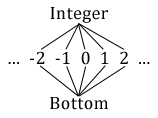
\includegraphics[width=0.25\textwidth]{images/integer-lattice.png}
	\end{center}
	\vspace{-15pt}
	\caption{The integer lattice}
	\label{fig:latticeInteger}
\end{figure}



\subsection{Abstract State}
We use the following lattice to model abstract state:

\begin{figure}[H]
\begin{equation*}
State = Heap \times Stack
\end{equation*}
\vspace{-15pt}
\caption{The $State$ lattice.}
\label{lattice:State}
\end{figure}

Before we describe the $Heap$ (\autoref{The Heap}) and $Stack$ (\autoref{The Stack}) lattices, we need to look at the $Object$ lattice:

\begin{figure}[H]
\begin{equation*}
Object = (AttributeName \rightarrow Value \times Global) \times P(ObjectLabel^{*})
\end{equation*}
\vspace{-15pt}
\caption{The $Object$ lattice.}
\label{lattice:Object}
\end{figure}

Having made special lattices for the 'primitive' objects there is still a need to handle the more complex objects such as class instances and function objects. As with JavaScript you can augment objects with attributes at runtime, so the lattice needs to accommodate this dynamic behavior. We therefore use a map from attribute names to values. For some objects it is required to track the scope in which they were defined, to model the closure they are evaluated in. Additionally, variable scope objects will be modeled with abstract values of this type, and here the ability to mark variables as global is needed, indicating that writes to this variable should be done in the global variable scope object. Thus the object lattice is the product between object values and a static scope chain modeled as a list of object labels. The static scope chain is only present for function objects and describes the scope of the function at its declaration. It is used to properly update the scope chain when calling the function.

\subsection{The Heap}
\label{The Heap}

\begin{figure}[H]
\begin{equation*}
Heap = (ObjectLabel \rightarrow Object)
\end{equation*}
\vspace{-15pt}
\caption{The $Heap$ lattice.}
\label{lattice:Heap}
\end{figure}

The heap is modeled by a map from object labels to object values. During the execution of a program there may be unbounded many objects on the heap, which we must approximate with a finite representation. We do this by using an object label for each allocation site, i.e. each node in the CFG that may create a new object on the heap. This is commonly known as the \textit{allocation-site abstraction} \cite{recency,aopas}, which we get back to in \autoref{section:Strong or weak}. Thus, our abstract heap lattice will only contain one object for each such allocation site.

As an illustrative example consider the following very simple program:

\begin{listing}[H]
	\begin{minted}[linenos]{python}
class C(): pass
x = []
for y in range(0,2):
  x.append(C())
x[0].a = 'a'
x[1].b = 'b'
	\end{minted}
	\caption{Imprecision introduced by allocation-site abstraction.}
\end{listing}

At runtime this example generates two different \inlinecode{C} objects with attributes \inlinecode{a} and \inlinecode{b}, respectively. Using the allocation-site abstraction only a single \inlinecode{C} object would be created on the abstract heap. As a consequence, when writing to the attribute \inlinecode{a} at line 5, this is in principle done on each object originating from the same allocation-site\footnote{In order to deal with this conservatively, it must of course be a weak update. We discuss strong and weak updates in \autoref{section:Strong or weak}.}. Thus an analysis for this code should conclude at the end that the attribute \inlinecode{a} of an object originating from line 4 might be undefined or \inlinecode{'a'} (similar for \inlinecode{b}).

As a side note we mention that the approach taken here is quite similar to the one taken in the Static Analysis course\footnote{See \url{http://cs.au.dk/SA}.}, where a couple of points-to analyses for Tiny Imperative Language (TIP) was described. There, \textit{Targets} was introduced as the possible set of allocations-sites, which for TIP is the pointer targets \inlinecode{malloc-i} for a given program (page 74, \cite{sa}).

In our type analyser we found it beneficial to distinguish between different types of object labels but still handle them in the same way in the heap. To achieve this we made several different subclasses to the object label, e.g. a function object label, which besides its name also holds a reference to the CFG node that is the entry node for that function.


\subsection{The Stack}
\label{The Stack}
The $Stack$ lattice is defined as:

\begin{figure}[H]
\begin{equation*}
Stack = (Register \rightarrow Value) \times P(ObjectLabel^{*})
\end{equation*}
\vspace{-15pt}
\caption{The $Stack$ lattice.}
\label{lattice:Stack}
\end{figure}

For each register, which can be thought of as a temporary variable, we specify the value of that particular register. Recall that we use registers in our intermediate representation, see \autoref{fig:callCfg} in \autoref{CFG calls} about CFG construction of function and method calls.

The power set $P(ObjectLabel^{*})$ specifies the objects on the dynamic scope chain $ObjectLabel^{*}$, i.e. the runtime stack. The head element in the scope chain determines which object on the heap, local variable writes should we written to. For instance we will have an object on the heap for each program, that models the module/top-level script environment \inlinecode{\_\_main\_\_} \cite{pyref.main} (this is what corresponds to the global object in JavaScript). Whenever an assignment to a variable occurs in the top-level scripting environment, e.g. \inlinecode{x=10}, the variable \inlinecode{x} is set as a attribute mapping to the integer 10 on the \inlinecode{\_\_main\_\_} object in the heap.

The dynamic scope chain is captured as the static scope chain whenever a class or function is declared. This new static scope chain is stored in the $Object$ lattice as seen in \autoref{lattice:Object}. The following example demonstrates this:

\begin{listing}[H]
	\begin{minted}[linenos]{python}
x = 10
def a():
  return x
a() # 10
x = 42
a() # 42
	\end{minted}
\caption{Scope example.}
\label{code:ScopeExample}
\end{listing}

For this example we will have the following objects on the abstract heap:

\begin{enumerate}
  \item The \inlinecode{\_\_main\_\_} object,
  \item The object of the function \inlinecode{a},
  \item The scope object of \inlinecode{a} (which is an object similar to the \inlinecode{\_\_main\_\_} object, i.e. an object where local variables are written onto).
\end{enumerate}

When calling the function the dynamic scope chain will be set to the static scope chain related to the function \inlinecode{a} in order to model Pythons static scoping. When the variable \inlinecode{x} is read, \inlinecode{x} is looked up in the scope chain; for this particular example \inlinecode{x} is found on the \inlinecode{\_\_main\_\_} object.

In the \autoref{Functions} we describe our work towards handling functions, this includes populating the call graph such that the CFG becomes interprocedural.

\begin{figure}[H]
\begin{eqnarray*}
CallGraph = & P(Node \times Node) \\
Analysis = & (Node \rightarrow State) \times CallGraph
\end{eqnarray*}
\vspace{-15pt}
\caption{The $CallGraph$ and $Analysis$ lattice.}
\label{lattice:Analysis}
\end{figure}